%% Campus-GPT IEEE conference draft (approx. 6--8 pages when compiled)
%% Overleaf: upload this folder; set main file to ieee_campus_gpt.tex
%% Compile twice with pdfLaTeX for references/cross-refs.
\documentclass[conference]{IEEEtran}
\IEEEoverridecommandlockouts

\usepackage{cite}
\usepackage{amsmath,amssymb,amsfonts}
\usepackage{algorithmic}
\usepackage{graphicx}
\usepackage{textcomp}
\usepackage{xcolor}
\usepackage{booktabs}
\usepackage{tabularx}
\usepackage{url}
\usepackage{hyperref}
\usepackage{enumitem}

\graphicspath{{figures/}}

\begin{document}

\title{Campus-GPT: A Policy-Aware and Privacy-Preserving AI Assistant for Personalized University Decision Support}

\author{
\IEEEauthorblockN{Author Name}
\IEEEauthorblockA{\textit{Department of Computer Science and Engineering}\\
\textit{Kalasalingam Academy of Research and Education (KARE), India}\\
email@klu.ac.in}
}

\maketitle

\begin{abstract}
University decision support spans institutional policy documents and highly sensitive personal academic records. Generative AI assistants that mix both sources without governance risk hallucination, unauthorized disclosure, and bypass of established enterprise workflows. This paper presents \emph{Campus-GPT}, a working prototype of a policy-aware, privacy-conscious AI layer integrated with a University Information System (UIS). The design treats UIS as the system of record (SoR) and Campus-GPT as a multi-agent assistant that answers institutional questions via retrieval-augmented generation (RAG) and personal questions only through a consent-gated integration API. Role-based access control (RBAC), partial attribute-based ownership checks (ABAC), and opt-in consent scopes jointly constrain data release. Heuristic response confidence (escalation threshold $\theta{=}0.7$) guides human escalation but is \textbf{not} reported as model accuracy. We describe the dual-system architecture, query pipeline, security controls, KARE demonstration environment, and an evaluation methodology for future measurement. Formal latency, retrieval (e.g., Precision@$k$), and answer-accuracy benchmarks are not yet available and remain future work.
\end{abstract}

\begin{IEEEkeywords}
Campus AI assistant, retrieval-augmented generation, university information system, consent, privacy, ABAC, multi-agent systems, Gemini, FAISS
\end{IEEEkeywords}

\section{Introduction}
Modern campuses operate fragmented portals for academics, hostel administration, fees, complaints, and notices. Students and staff need timely answers that combine \emph{policy knowledge} (handbooks, circulars, FAQs) with \emph{personal records} (attendance, marks, leave status). Large language models (LLMs) can reduce navigation friction, yet naive deployments often (i)~invent personal numbers, (ii)~over-retrieve documents without citations, or (iii)~expose ERP data without purpose limitation~\cite{lewis2020rag,kasneci2023chatgpt}.

We therefore propose a \textbf{general university framework}---demonstrated at Kalasalingam Academy of Research and Education (KARE)---that separates the enterprise SoR from the AI interaction layer. UIS remains authoritative for structured workflows; Campus-GPT provides conversational decision support under explicit policy and privacy constraints.

\textbf{Positioning.} This paper describes a \emph{working prototype}, not an experimentally proven superior architecture. Claims are architectural and functional; numerical model accuracy is not asserted.

\textbf{Contributions.}
\begin{enumerate}[leftmargin=*,itemsep=1pt]
  \item A dual-system UIS~+~AI architecture with schema isolation and a controlled integration contract.
  \item Consent-gated personal-data assembly combined with RBAC and ownership-oriented ABAC checks.
  \item Multi-agent desks that change persona, session context, and topic guardrails without swapping the underlying LLM.
  \item Policy-aligned workflows (e.g., dual-approval hostel leave) that keep write authority in UIS.
  \item An evaluation methodology for latency, retrieval quality, and answer correctness \emph{without inventing results}.
\end{enumerate}

\section{Related Work}
RAG improves grounding for knowledge-intensive tasks by retrieving evidence before generation~\cite{lewis2020rag}. Higher-education GenAI surveys highlight opportunities and risks around assessment integrity, privacy, and institutional adoption~\cite{kasneci2023chatgpt,yan2024practical}. Campus chatbots historically relied on FAQ trees or closed domains; recent systems couple LLMs with campus knowledge bases but often under-specify SoR boundaries. Access control literature distinguishes RBAC from ABAC~\cite{hu2014guide}; practical campus systems usually combine role gates with resource ownership. Our prototype aligns with privacy-by-design: deny-by-default consent for personal scopes and audited integration reads.

\section{System Overview}
\subsection{Dual-application topology}
Fig.~\ref{fig:arch} shows the complete Campus-GPT + UIS architecture. UIS (Next.js UI, FastAPI API) exposes ERP portals. Campus-GPT (Next.js UI, FastAPI API) hosts chat, RAG, voice, and admin tools. In the KARE demonstration environment, local ports are UIS UI~3000 / API~8000 and Campus-GPT UI~3001 / API~8002. Campus-GPT never mounts the UIS database; it calls \texttt{/api/v1/integration/campus-gpt/*} with a shared API key and a user JWT.

\begin{figure}[!t]
\centering
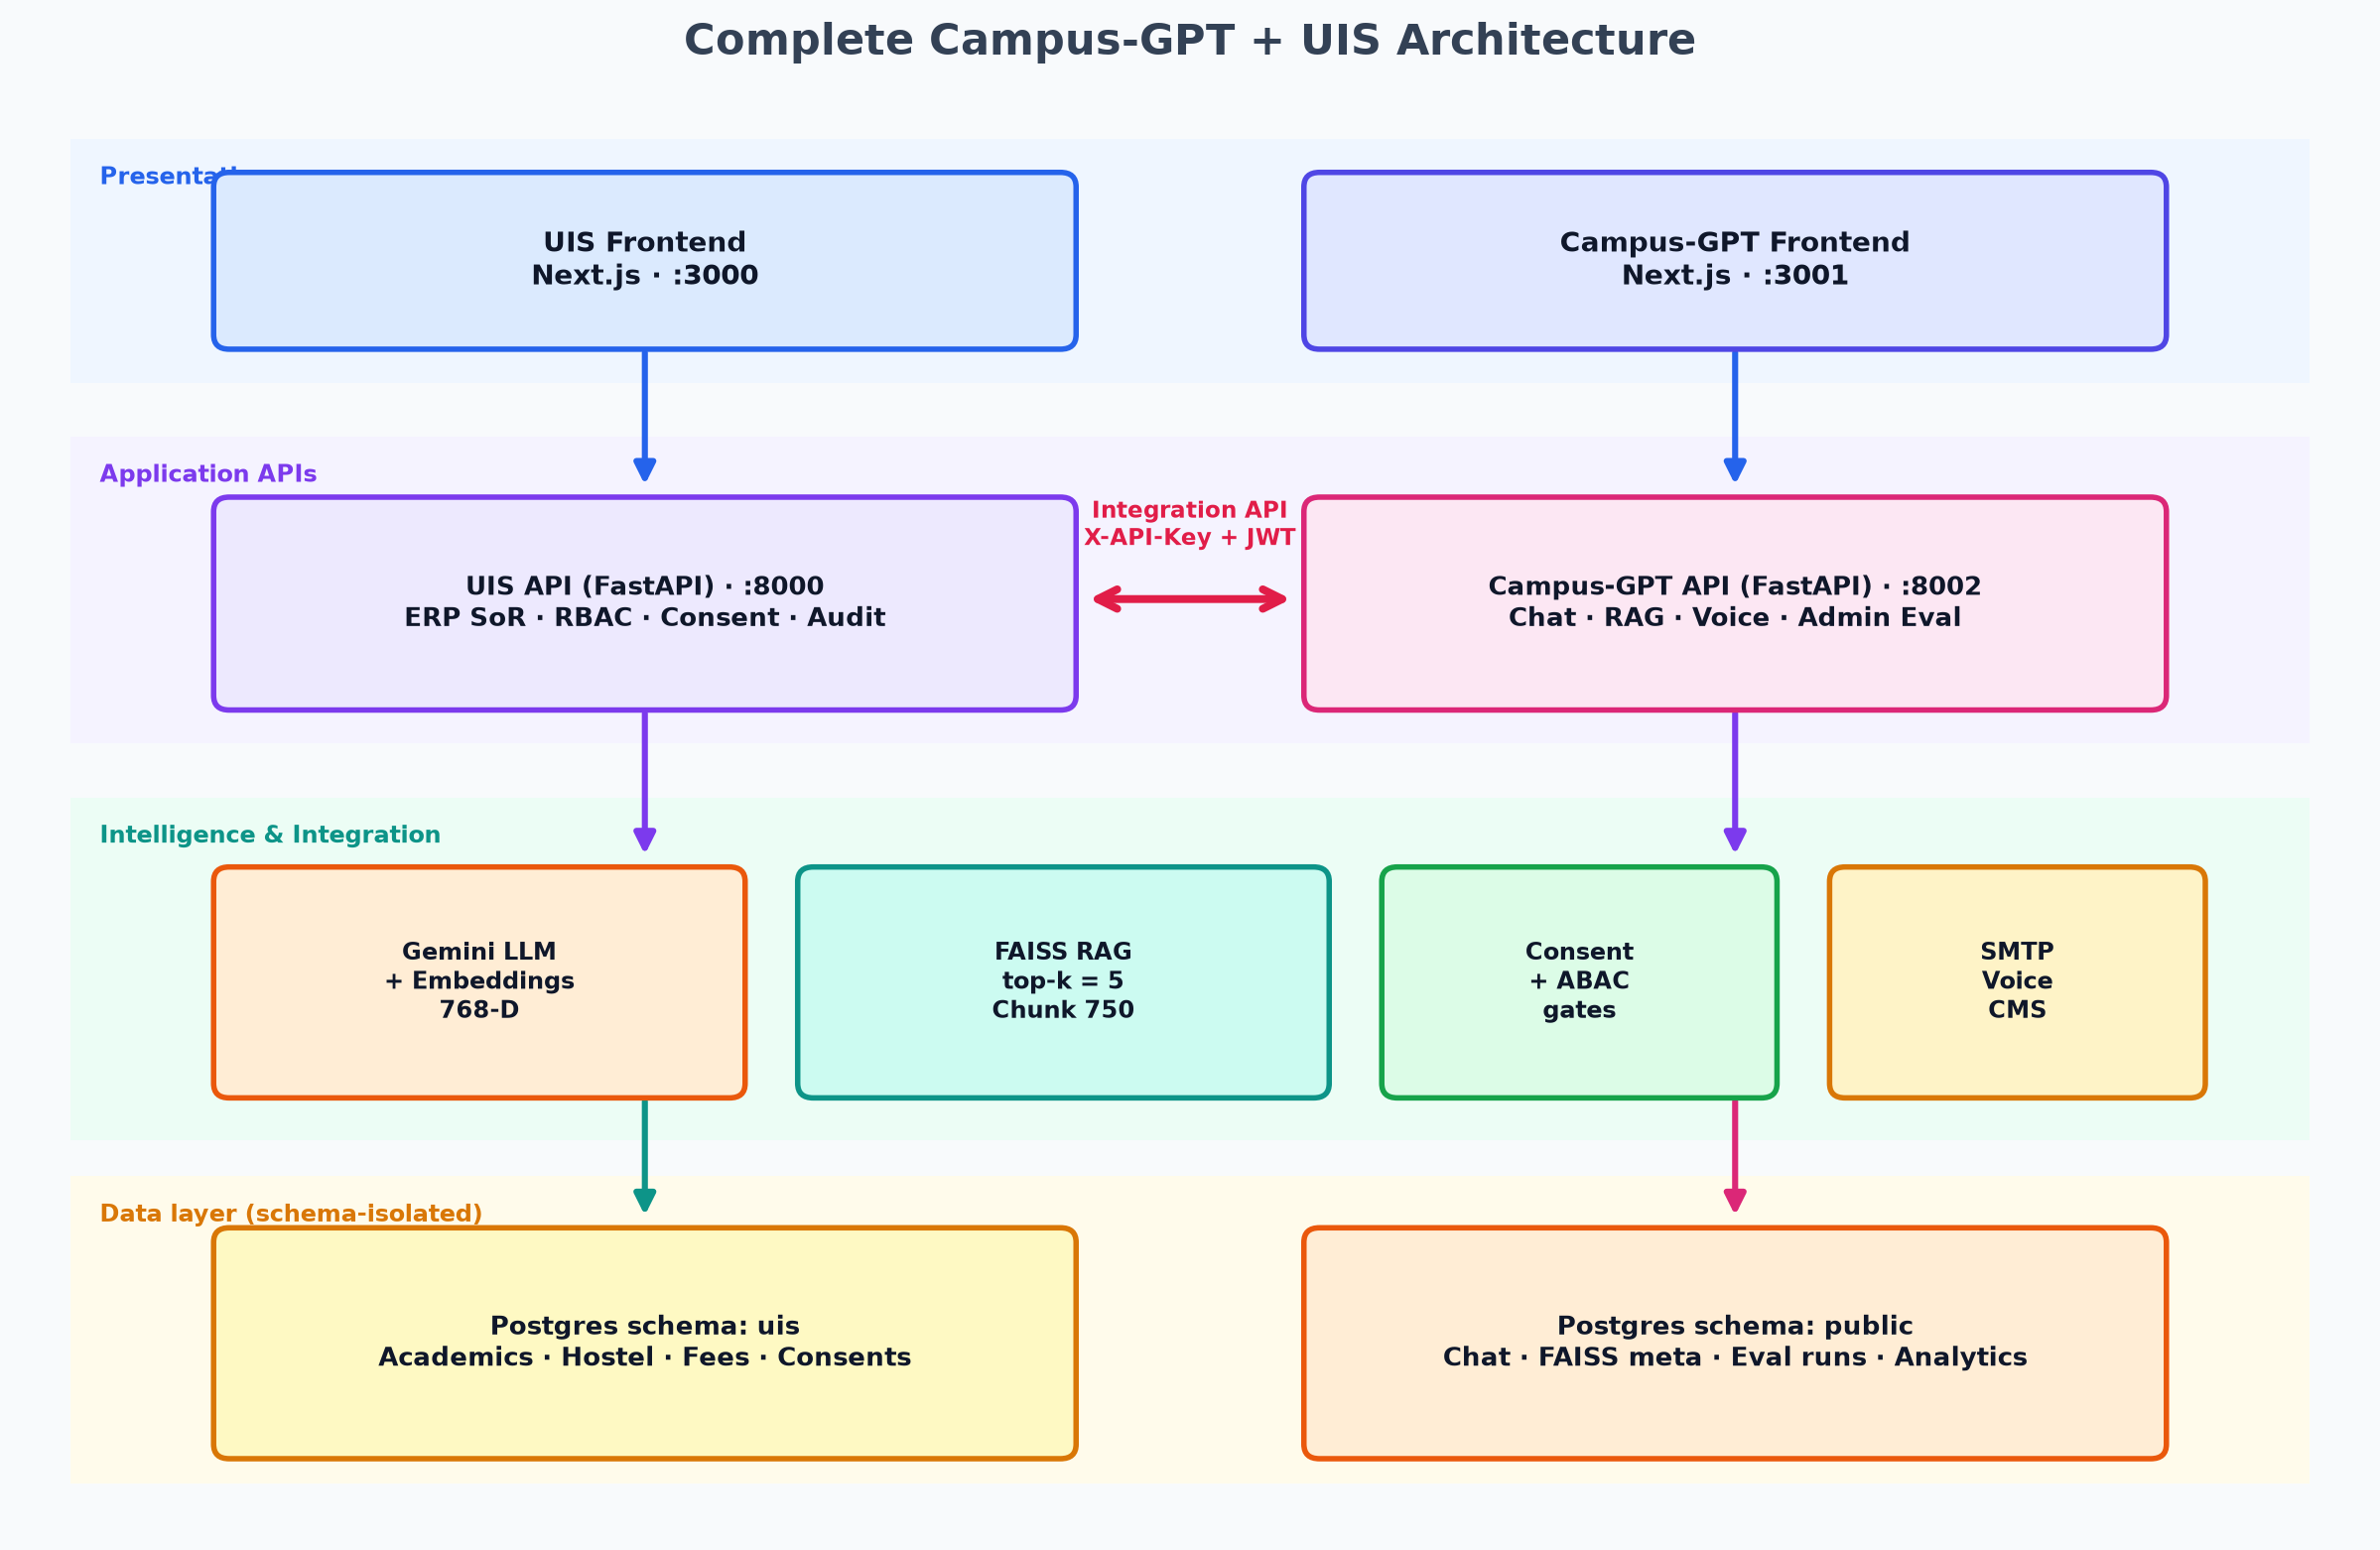
\includegraphics[width=\columnwidth]{fig1_architecture.png}
\caption{Complete Campus-GPT + UIS architecture with presentation, API, intelligence, and schema-isolated data layers.}
\label{fig:arch}
\end{figure}

\subsection{Schema isolation}
Both applications may share one Postgres project (e.g., Supabase). Campus-GPT tables reside in schema \texttt{public}; UIS tables reside in schema \texttt{uis}. This avoids colliding user models and clarifies data ownership for backups and access reviews.

\section{Privacy, Consent, and Access Control}
\subsection{Consent-gated personal data}
Personal scopes (examples: \texttt{academic.attendance}, \texttt{hostel.leave}, \texttt{fees.records}, \texttt{messaging.inbox}) are stored in UIS \texttt{integration\_consents} and default to deny until the student opts in. Denied scopes yield HTTP~403 (\texttt{CONSENT\_DENIED}) and are audited.

\subsection{RBAC and partial ABAC}
RBAC gates portals and administrative APIs by role. Ownership-oriented ABAC is implemented in code for selected paths: integration queries are bound to the authenticated subject's student identity; attempts to request another student's marks via \texttt{target\_student\_id} are rejected and audited as \texttt{DENIED\_ABAC}; faculty class operations assert assigned-offering membership. This is a practical ABAC fragment, not a full XACML/OPA policy engine.

\subsection{Authentication}
Sessions use JWT (HS256). In the KARE deployment, Google OAuth may be restricted to the institutional domain \texttt{klu.ac.in}. Credentials are preferentially verified against UIS and linked via \texttt{uis\_username}.

\section{Query Processing and Multi-Agent Behavior}
\subsection{End-to-end workflow}
Fig.~\ref{fig:workflow} summarizes end-to-end query processing. After authentication and agent selection, Campus-GPT enforces desk scope, attempts structured UIS assembly when consent allows (Fig.~\ref{fig:raguis}), otherwise retrieves FAISS chunks, then generates with Gemini. Confidence below $\theta{=}0.7$ may escalate.

\begin{figure}[!t]
\centering
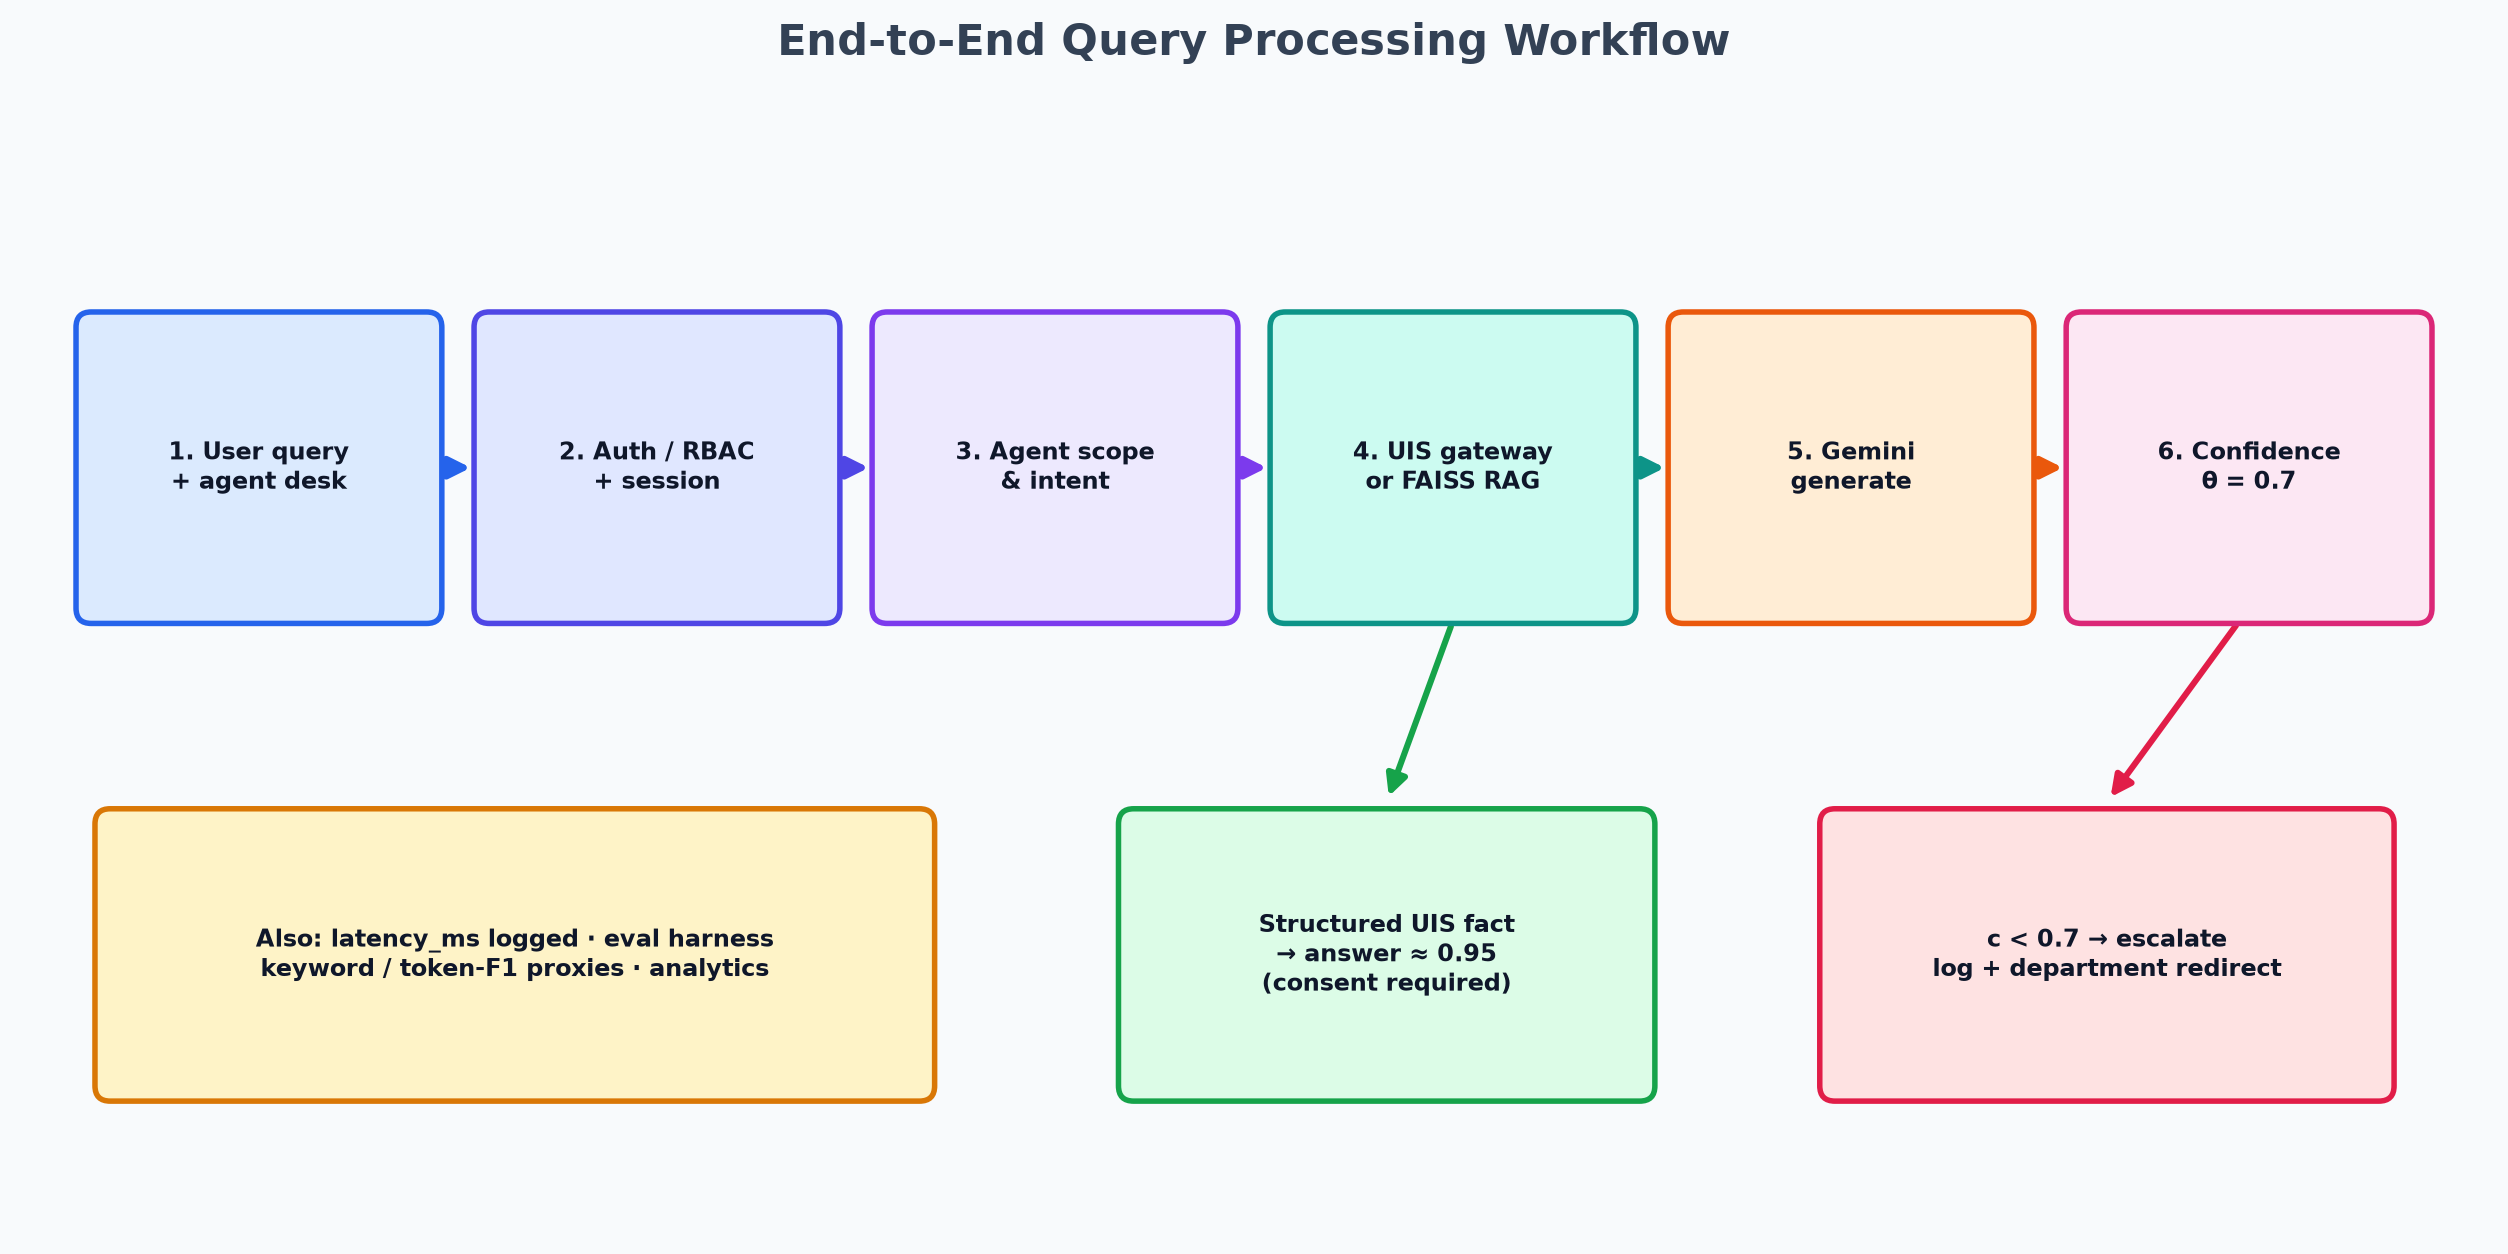
\includegraphics[width=\columnwidth]{fig2_query_workflow.png}
\caption{End-to-end query processing workflow from user input through confidence/escalation.}
\label{fig:workflow}
\end{figure}

\begin{figure}[!t]
\centering
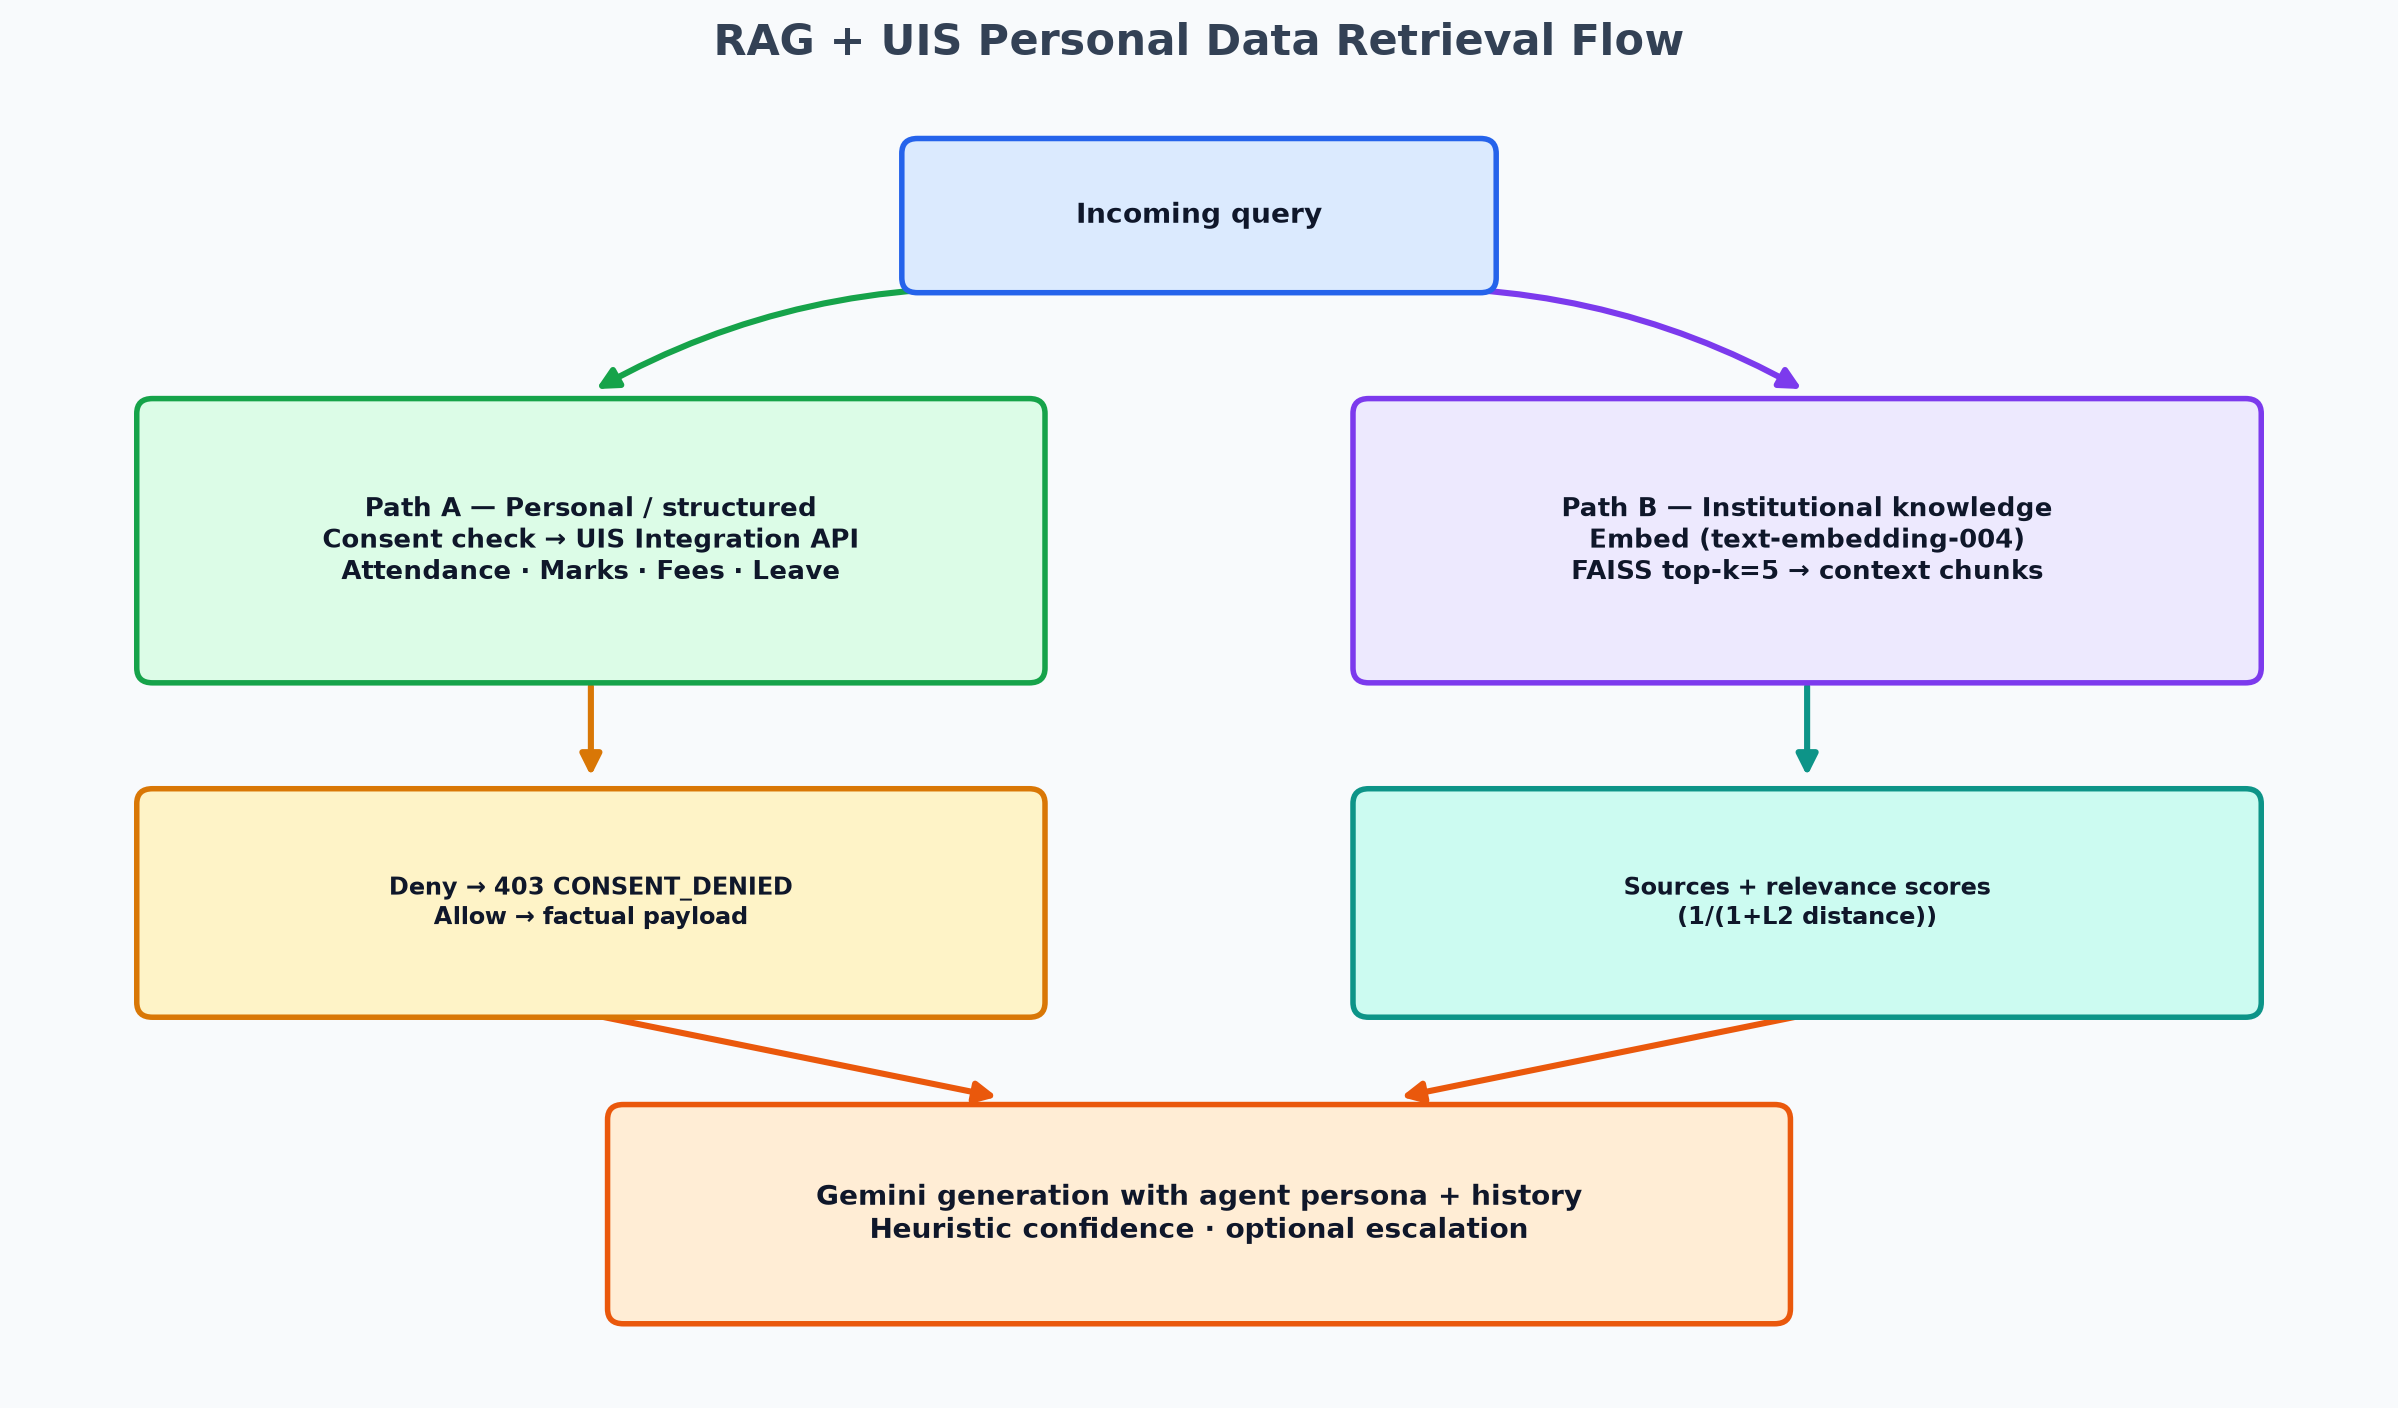
\includegraphics[width=\columnwidth]{fig3_rag_uis_flow.png}
\caption{RAG path for institutional knowledge versus consent-gated UIS retrieval for personal structured data.}
\label{fig:raguis}
\end{figure}

\subsection{Agent selection UI}
Fig.~\ref{fig:agents} illustrates the Campus-GPT multi-agent selection surface (Campus Guide, Academic, Faculty, Admission, Reception, Hostel, Warden). Selecting an agent changes UI theme, suggested queries, chat session isolation, LLM persona, and topic guardrails---not the base model or FAISS index.

\begin{figure}[!t]
\centering
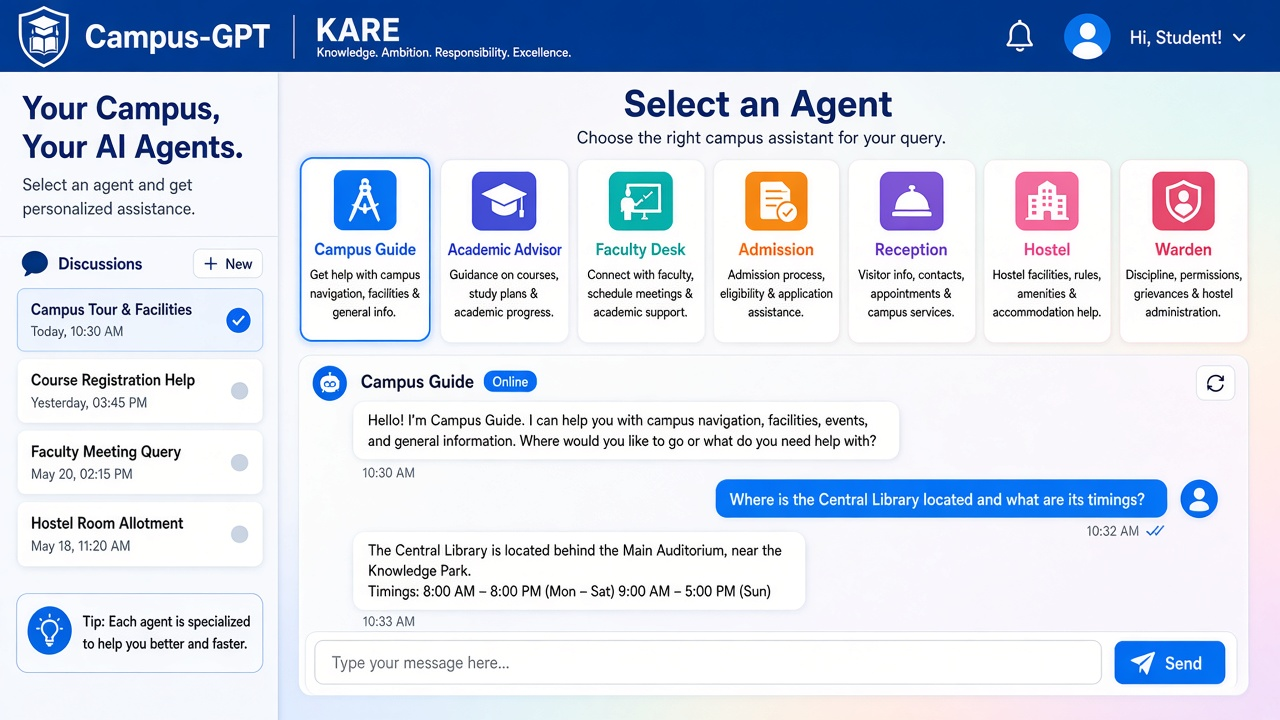
\includegraphics[width=\columnwidth]{fig4_agent_selection_ui.png}
\caption{Campus-GPT chat UI with colorful multi-agent desk selection.}
\label{fig:agents}
\end{figure}

\subsection{What changes when an agent is selected}
Selecting an agent changes: (1)~UI theme and suggested queries; (2)~chat session isolation (separate histories); (3)~LLM persona string; (4)~topic guardrails (hostel/warden refuse non-hostel questions); (5)~preferred action paths (e.g., leave proposals). It does \textbf{not} change the base LLM, embedding model, FAISS index, user identity, or consent store.

\subsection{Models and retrieval parameters}
\begin{itemize}[leftmargin=*,itemsep=1pt]
  \item Chat: Gemini \texttt{gemini-flash-latest} (temperature $0.2$; configured fallbacks available).
  \item Embeddings: \texttt{text-embedding-004}, dimension $768$.
  \item Vector index: FAISS \texttt{IndexFlatL2}; top-$k{=}5$; chunk size $750$; overlap $100$.
  \item Voice (optional): ElevenLabs STT/TTS with Whisper / edge-tts fallbacks.
\end{itemize}

\subsection{Heuristic confidence (not accuracy)}
The prototype assigns \emph{heuristic} confidence scores for escalation routing:
\begin{align}
c_{\text{UIS}} &\approx 0.95, \quad
c_{\text{RAG}} \approx 0.85, \quad
c_{\text{weak}} \approx 0.3, \\
\text{escalate} &\iff (c < \theta)\;\wedge\;\text{enabled},\quad \theta = 0.7.
\end{align}
These values are design-time heuristics encoded in software. They must \textbf{not} be interpreted as validated accuracy, Precision@$k$, or human-judged correctness.

\section{University Information System Capabilities}
UIS implements the SoR modules used by Campus-GPT: departments/programs/courses, enrollments, attendance, marks/grades, timetable, examinations, hostel allocations, dual-approval leave (faculty + warden), fees, complaints, messaging, announcements/marquee, and branding CMS.

\section{Implementation Stack}
Table~\ref{tab:stack} summarizes technologies used in the working prototype.

\begin{table}[!t]
\renewcommand{\arraystretch}{1.12}
\caption{Implementation stack (KARE demonstration prototype)}
\label{tab:stack}
\centering
\begin{tabular}{p{0.18\columnwidth}p{0.36\columnwidth}p{0.36\columnwidth}}
\toprule
\textbf{Layer} & \textbf{UIS} & \textbf{Campus-GPT} \\
\midrule
UI & Next.js~14, React~18, TypeScript, Tailwind & Next.js~14, React~18, TypeScript, Tailwind \\
API & FastAPI, Uvicorn & FastAPI, Uvicorn \\
Data & SQLAlchemy~2, Postgres schema \texttt{uis} & SQLAlchemy~2, Postgres schema \texttt{public} \\
AI & --- & Gemini, FAISS, optional Whisper/TTS \\
Security & JWT, bcrypt, consent, audit & JWT, OAuth domain gate, consent client \\
\bottomrule
\end{tabular}
\end{table}

\section{Evaluation Methodology and Measurement Capability}
\subsection{Instrumentation in the working prototype}
The Campus-GPT application now records end-to-end chat latency (\texttt{latency\_ms}) on each \texttt{/api/chat} call and provides an administrator evaluation harness:
\begin{itemize}[leftmargin=*,itemsep=1pt]
  \item \textbf{Live latency:} average, minimum, maximum, and median from \texttt{query\_logs}.
  \item \textbf{Gold suite run:} institutional FAQ cases in \texttt{app/eval/gold\_set.json} executed through \texttt{rag\_pipeline}.
  \item \textbf{Automatic answer proxies:} keyword hit-rate against expected keywords; token-overlap F1 against a reference answer.
  \item \textbf{Retrieval proxy:} keyword-in-sources hit@$k$ (not annotated Precision@$k$/Recall@$k$).
\end{itemize}
Administrators trigger runs via \texttt{POST /api/admin/eval/run} or the Evaluation UI. Results are persisted in \texttt{eval\_runs} / \texttt{eval\_case\_results}.

\subsection{What has not been claimed without measurement}
Until a gold run is executed and reported, this paper does \textbf{not} publish fabricated averages. Prior to instrumentation, only database health pings existed. Formal human evaluation, Exact Match on personal facts, and IR Precision@$k$/Recall@$k$ with chunk annotations remain future work.

\subsection{Prototype evaluation stance}
In addition to the harness, the prototype was validated through \textbf{functional and security test scenarios}: authentication and role shells; consent allow/deny; ABAC rejection of cross-student marks; hostel desk off-topic refusal; dual-approval leave; and RAG over uploaded documents. These validate behavior and controls.

\subsection{Reporting guidance}
When publishing numbers, report: (i)~suite name and case count, (ii)~latency avg/min/max/median, (iii)~keyword accuracy and token F1 as \emph{automatic proxies}, (iv)~explicit disclaimer that proxies are not human-rated accuracy.

\section{Limitations and Future Work}
Limitations include heuristic (uncalibrated) confidence, dependence on UIS availability, optional third-party voice services, and demonstration seed data. Future work includes calibrated confidence, hybrid sparse--dense retrieval with re-ranking, multilingual campus support, production payment gateways, stronger data-protection retention controls, distributed tracing, and a public evaluation dataset for campus RAG.

\section{Conclusion}
Campus-GPT demonstrates a working prototype of a policy-aware, privacy-preserving AI assistant for personalized university decision support. By pairing RAG over institutional knowledge with a consent-gated UIS integration, isolating schemas, and applying RBAC together with ownership ABAC checks, universities can adopt generative AI without surrendering ERP integrity. The scientifically appropriate claim today is architectural and functional; formal accuracy, retrieval, and latency benchmarks remain essential next steps.

\section*{Acknowledgment}
The authors thank KARE for serving as the implementation and demonstration environment, and the communities maintaining FastAPI, Next.js, FAISS, and the Gemini API.

\begin{thebibliography}{00}

\bibitem{lewis2020rag}
P.~Lewis \emph{et~al.}, ``Retrieval-augmented generation for knowledge-intensive NLP tasks,'' in \textit{Proc.\ NeurIPS}, 2020.

\bibitem{kasneci2023chatgpt}
E.~Kasneci \emph{et~al.}, ``ChatGPT for good? On opportunities and challenges of large language models for education,'' \textit{Learning and Individual Differences}, vol.~103, 2023.

\bibitem{yan2024practical}
L.~Yan \emph{et~al.}, ``Practical and ethical challenges of large language models in education: A systematic scoping review,'' \textit{British Journal of Educational Technology}, vol.~55, no.~1, pp.~90--112, 2024.

\bibitem{hu2014guide}
V.~C.~Hu \emph{et~al.}, ``Guide to Attribute Based Access Control (ABAC) Definition and Considerations,'' NIST SP 800-162, 2014.

\bibitem{johnson2019billion}
J.~Johnson, M.~Douze, and H.~J\'{e}gou, ``Billion-scale similarity search with GPUs,'' \textit{IEEE Trans.\ Big Data}, vol.~7, no.~3, pp.~535--547, 2021.

\bibitem{openai2023gpt}
OpenAI, ``GPT-4 Technical Report,'' arXiv:2303.08774, 2023.

\bibitem{gemini2024}
Google DeepMind, ``Gemini: A Family of Highly Capable Multimodal Models,'' 2024. [Online]. Available: \url{https://ai.google.dev}

\bibitem{fastapi}
S.~Ram\'{i}rez, ``FastAPI documentation,'' 2024. [Online]. Available: \url{https://fastapi.tiangolo.com}

\end{thebibliography}

\end{document}
